
%----------------------------------------------------------------------------------------
%	Lecture 3
%----------------------------------------------------------------------------------------

\chapter{Level Curves, Partial Derivative and Tangent Planes}

\bigbreak
\section{Level Curves}

\subsection{Multivariate Functions}

If a function depends on more than one variable then it is called a Multivariate function.
We will focus mostly on functions that depend on two variable $x$ and $y$.
We plot such functions in xyz-space by setting $z = f(x, y)$ so the height of a point at $(x, y)$ is the value of the function on that point.

\subsection{Level Curves}

The level curve of a function $f(x, y)$ are all the points where $f(x, y)$ is equal to some constanc $c$.
Its like a map telling you how high things are at some point.
To plot this, we can slice the graph by horizontal planes. 


\begin{figure}[ht!]
    \centering
    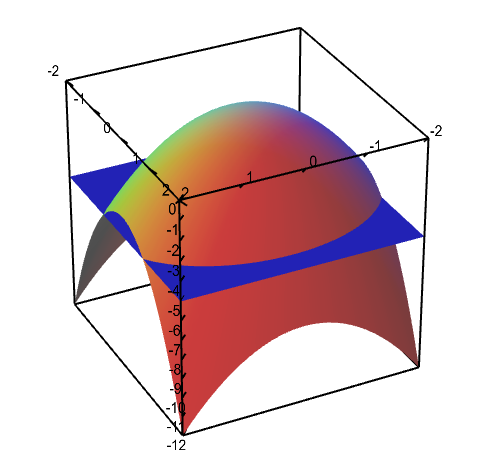
\includegraphics[scale=0.5]{./images/lecture_3_figure_1.png}
    \caption{Level Curve for a function using a horizontal slice}
\end{figure}

Level curves for both increasing and decreasing functions look the same so that's why they need to be marked with values.
Level curve make it easier to determine whether the function increases or decreases in a particular direction.


\subsection{Partial Derivatives}

A partial derivative is when we change only on variable and don't change the other variables.
$$ \px{f}{x} = \lim_{\Delta x \to 0} \frac{f(x+\Delta x, y) - f(x, y)}{\Delta x} $$

Geometrically, it means that we take a point $(x, y)$ and change $x$ a little, keeping $y$ constant.
Keeping $y$ constant means that we're moving parallel to the X-axis which gives us a curve in the XZ-plane.
And the partial derivative of the function is the slope of that curve at $(x, y)$.
Another notaion for \ilds{\px{f}{x}} is $f_x$ and \ilds{\px{f}{y}} is $f_y$.


{\bf Example : } Let $f(x, y) = x^3 y  + y^2$ then $f_x = 3x^2y$ and $f_y = x^3 + 2y$.

\subsection{Tangent Planes}

From the above definition of the partial derivative, we can say that $f_x$ and $f_y$ are the slopes of the lines tangent to the curve $f(x, y)$ at the point $(x ,y)$.
If we have two lines tangent to the surface then we can determine the plane tangent to the surface.

If $f_x(x_0, y_0) = a$, then the line is defined by $y = y_0$ and $z = z_0 + a(x-x_0)$ since this line is in the XZ-plane.

If $f_y(x_0, y_0) = b$, then the line is defined by $x = x_0$ and $z = z_0 + b(y-y_0)$ since this line is in the YZ-plane.

Both the lines are going to be in the tangent plane of the surface. So together the determine the plane. 
That plane is given by the formula $z = z_0 + a(x-x_0) + b(y-y_0)$.

You can also determine the plane by taking cross product of the vectors along the line and finding the normal vector of the plane. 
That will give you the same formula.


{\bf Approximation Formula : } $\Delta f = f_x (\Delta x) + f_y (\Delta y)$.